\scanpage{15}
\begingroup
\makeatletter
\tagsleft@true
\makeatother
\uline{\deleted{\unsure{I|V}}Version I}

% G01: detached short dot at full-scan (190,140)--(196,147); hand, role and surface origin undetermined.
\reversemarginpar
\margin{\unsure{$\cdot$}}
\normalmarginpar
Soient $X$ un espace topologique, $(\deleted{\unsure{\Sigma|S}}E_i)_{i\in I}$ un ens. de
% Opening local group; coordinates are full scan minus (195,169).
\figure{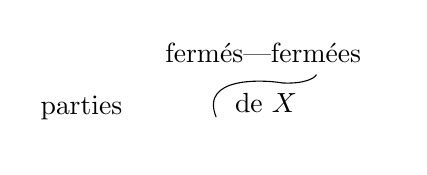
\begin{tikzpicture}[x=.013cm,y=-.013cm,line cap=round,line join=round]
\path[use as bounding box] (0,0) rectangle (363,116);
\node[anchor=base west,inner sep=0] at (12,85) {parties};
\node[anchor=base west,inner sep=0] at (134,34) {\inserted{\unsure{fermés|fermées}}};
\node[anchor=base west,inner sep=0] at (202,83) {de $X$};
% GUIDE01: the curved insertion guide, (379,256) to (477,215) on the full scan.
\draw (184,87) .. controls (168,47) and (232,51) .. (249,54)
 .. controls (269,55) and (280,50) .. (282,46);
\end{tikzpicture}}
(noté indiciellement), telles que l'on ait
% slanted
\reversemarginpar
\margin{$\nearrow$ On suppose de plus que pour \unsure{tte|toute|tt} comp. conn. $\Sigma_i$ de $X\setminus E_i$, on ait $\overline{\Sigma}_i\cap E_i\ne\varnothing$ i.e. $\overline{\Sigma}_i\ne\Sigma_i$ i.e. $\Sigma_i$ non fermé dans $X$ (ce qui est le cas si $X$ est connexe)}
\normalmarginpar
\[
 \forall i\in I,\quad \operatorname{Card}\pi_0(X\setminus\deleted{\Sigma}E_i)=2
 \tag*{(a)}
\]
% G02: separate upper horizontal stroke over the first Sigma in this NB.
% The overset rule preserves the stroke; its role remains undetermined.
\margin{\uline{NB} les comp. conn. $\overset{\unsure{\rule{.8em}{.35pt}}}{\Sigma}_i^+,\Sigma_i^{\unsure{+|-|\ast}}$ de $X\setminus\Sigma_i$ sont ouvertes dans $X$}
\[
 \begin{aligned}
 &\forall(i,j)\in I\times I,\ i\ne j,\quad \deleted{\Sigma}E_j\ \text{est contenu dans l'une}\\
 &\text{des deux composantes connexes de }X\setminus\deleted{\Sigma}E_i.
 \end{aligned}
 \tag*{(b)}
\]

NB Cette condition (b) est vérifiée automatiquement les $\deleted{\Sigma}E_i$ $(i\in I)$ sont connexes, dès lors que les $E_i$ sont supposés disjoints mutuellement

On se propose d'étudier le ``découpage'' de $X$ par la famille $(E_i)$.

% The heading underline has a separate short run beneath 2.
\uline{Cas $\operatorname{Card}\deleted{\unsure{(\mathrm{de})}}(I)\deleted{\unsure{\leq|=}}=$}\ \uline{$2$}

Soit $\Sigma_i^+$ la comp. conn. de $X\setminus E_i$ qui ne contient pas $E_j$ $(j\ne i)$, alors on a (si $I=\{1,2\}$)
% Drawing coordinate map: full-scan (x,y) = local (x+22,y+1069).
% The pale lower-right rim is drawn in separate supported runs; its exact continuity remains uncertain.
\figure{\begin{tikzpicture}[x=.013cm,y=-.013cm,line cap=round,line join=round]
\path[use as bounding box] (0,-40) rectangle (535,300);
\draw (182,89) .. controls (226,-13) and (337,-39) .. (379,72)
 .. controls (407,148) and (405,201) .. (388,217);
\node[anchor=north west,inner sep=0] at (354,222) {\unsure{\begin{tikzpicture}[x=.013cm,y=-.013cm,line cap=round]
\path[use as bounding box] (0,0) rectangle (34,44);
\draw[gray,line width=.28pt] (29,3) .. controls (24,17) and (15,29) .. (5,39);
\end{tikzpicture}}};
\draw (355,266) .. controls (341,275) and (321,280) .. (303,281)
 .. controls (217,298) and (139,247) .. (161,158)
 .. controls (157,176) and (155,135) .. (182,89);
\draw[line width=.8pt] (181,89) .. controls (256,91) and (313,77) .. (382,86)
 (174,218) .. controls (240,224) and (317,212) .. (380,212);
\draw (44,9) .. controls (46,57) and (63,106) .. (32,108)
 .. controls (52,132) and (38,151) .. (46,195) -- (55,228);
\draw (41,109) .. controls (72,143) and (35,144) .. (48,193)
 .. controls (47,224) and (57,241) .. (39,252) .. controls (55,242) and (43,259) .. (49,282);
\draw (428,86) .. controls (439,93) and (409,141) .. (434,149)
 .. controls (420,158) and (436,251) .. (417,254);
\node[inner sep=0] at (166,20) {\rlap{$\unsure{\Sigma_1^+|\Sigma_2^+}$}\phantom{$\deleted{\unsure{\Sigma_1^+|\Sigma_2^+}}$}};
% CANCEL01: the two diagonal crossing runs of the upper-left deleted label.
\draw[line width=.7pt] (135,39) -- (187,-8);
\draw[line width=.45pt] (141,32) .. controls (158,13) and (164,2) .. (177,-13);
\node at (139,90) {$E_1$}; \node at (149,220) {$E_2$};
\node at (429,32) {$\Sigma_1^+$};
\node at (492,160) {$\Sigma_1^{\deleted{\unsure{+}}\unsure{-}}$};
% G03: detached dot above the crowded right-hand exponent; role and hand undetermined.
\node[inner sep=0] at (507,125) {\unsure{$\cdot$}};
\node at (14,111) {$\Sigma_2^-$}; \node at (115,278) {$\Sigma_2^+$};
\end{tikzpicture}}
\[
 \Sigma_1^+\cap\Sigma_2^+=\varnothing
 \tag*{(1)}
\]
ce qui \deleted{résulte de} équivaut à
\[
 \begin{aligned}
 &\deleted{\Sigma_1^-\supset\Sigma_2^+}\\
 &\deleted{\Sigma_2^-\supset\Sigma_1^+}\qquad \Sigma_1^+\subset\Sigma_2^-\cup E_2,\quad\text{et}
 \end{aligned}
\]
% Local cancelled words, origin (211,1427); both horizontal crossing runs retained.
\figure{
\begin{tikzpicture}[x=.013cm,y=-.013cm,line cap=round]
\path[use as bounding box] (0,0) rectangle (220,86);
\node[anchor=base west,inner sep=0] at (15,57) {\rlap{\unsure{Car si|car si}}\phantom{\deleted{\unsure{Car si|car si}}}};
\draw (37,48) .. controls (90,46) and (138,45) .. (182,47);
\draw (45,54) .. controls (108,55) and (156,58) .. (201,58);
\end{tikzpicture}}
\deleted{Si on avait} comme $\Sigma_1^+\cap E_2=\varnothing$, cela équivaut aussi à
\[
 \Sigma_1^+\subset\Sigma_2^-
 \tag*{(2)}
\]
% G04: two detached small marks at full-scan (1602,1779)--(1612,1791); hand and role undetermined.
\margin{\unsure{\begin{tikzpicture}[x=.02cm,y=-.02cm]
\path[use as bounding box] (0,0) rectangle (10,12);
\fill (6,1) ellipse (1 and .7);
\fill (1,8) ellipse (1 and .6);
\end{tikzpicture}}}
\unsure{et} symétriquement, à
\[
 \Sigma_2^+\subset\Sigma_1^-
 \tag*{$(2')$}
\]

% Lower correction group: full-scan (x,y) = local (x+219,y+2009).
\figure{\begin{tikzpicture}[x=.009cm,y=-.009cm,line cap=round,line join=round]
\path[use as bounding box] (0,0) rectangle (1448,145);
\node[anchor=base west,inner sep=0] at (19,122) {Comme};
\node[anchor=base west,inner sep=0] at (207,43) {\rlap{\unsure{vois. ouvert}}\phantom{\deleted{\unsure{vois. ouvert}}}};
\draw (209,37) .. controls (270,33) and (334,38) .. (410,36);
\node[anchor=base west,inner sep=0] at (265,122) {$\Sigma_2^-\supset E_1,$};
% G05: detached slant below the struck words, visible (510,2076)--(526,2063).
\node[inner sep=0] at (299,61) {\unsure{\begin{tikzpicture}[x=.009cm,y=-.009cm,line cap=round]
\path[use as bounding box] (0,0) rectangle (16,13);
\draw (0,13) .. controls (5,6) and (10,1) .. (16,0);
\end{tikzpicture}}};
\node[anchor=base west,inner sep=0] at (556,97) {\rlap{il contient les}\phantom{\deleted{il contient les}}};
\draw (557,91) .. controls (705,95) and (858,86) .. (997,82);
\node[anchor=base west,inner sep=0] at (557,49) {\inserted{i.e. $\Sigma_2^-$ est un \uline{vois.} ouvert de $E_1$,}};
\node[anchor=base west,inner sep=0] at (1048,93) {on a};
\end{tikzpicture}}
% slanted
\reversemarginpar
\margin{$\overline{\Sigma_1^+}\cap E_1\ne\varnothing$ i.e. $\overline{\Sigma_1^+}\ne\Sigma_1^+$ \unsure{à signaler|à sign.ler} avant
% G06: curved detached guide; full-scan origin (180,2145), role of the curve undetermined.
\figure{\begin{tikzpicture}[x=.012cm,y=-.012cm,line cap=round]
\path[use as bounding box] (0,0) rectangle (124,78);
\node[inner sep=0] at (62,39) {\unsure{\begin{tikzpicture}[x=.012cm,y=-.012cm,line cap=round]
\path[use as bounding box] (0,0) rectangle (124,78);
\draw (9,69) .. controls (-1,38) and (49,35) .. (75,23)
 .. controls (102,16) and (119,12) .. (119,6);
\end{tikzpicture}}};
\end{tikzpicture}}}
\normalmarginpar
\[
 \Sigma_2^-\cap\Sigma_1^+\ne\varnothing
\]
Car $\underline{\overline{\Sigma_1^+}\cap E_1}\ne\varnothing$
% Final local insertion: coordinates are full scan minus (1278,2080).
\figure{\begin{tikzpicture}[x=.013cm,y=-.013cm,line cap=round,line join=round]
\path[use as bounding box] (0,0) rectangle (362,164);
\node[anchor=base west,inner sep=0] at (19,127) {(sinon};
\node[anchor=base west,inner sep=0] at (170,62) {\inserted{l'ouvert}};
\node[anchor=base west,inner sep=0] at (213,131) {$\Sigma_1^+$};
% GUIDE02: bent attachment guide from before Sigma to the right of the inserted word.
\draw (183,117) .. controls (207,63) and (230,75) .. (262,78)
 .. controls (285,81) and (311,79) .. (326,74) -- (326,70) -- (322,70);
\end{tikzpicture}}
serait \inserted{\unsure{un|une}} fermé dans $X$, donc
% Final deleted group: origin (928,2238). The detached upper remnants have no assigned character.
\figure{\begin{tikzpicture}[x=.013cm,y=-.013cm,line cap=round,line join=round]
\path[use as bounding box] (0,0) rectangle (165,67);
\node[anchor=base west,inner sep=0] at (21,49) {\rlap{\unsure{$\Sigma_1^+$ serait}}\phantom{\deleted{\unsure{$\Sigma_1^+$ serait}}}};
\draw (11,28) -- (51,5);
\draw (20,35) -- (70,13);
% G07: upper remnant cluster, shape retained locally under doubt; hand, role and surface origin undetermined.
\node[inner sep=0] at (28,14) {\unsure{\begin{tikzpicture}[x=.013cm,y=-.013cm,line cap=round]
\path[use as bounding box] (0,0) rectangle (37,24);
\draw (3,18) .. controls (11,8) and (8,7) .. (10,3) -- (15,18) -- (33,9);
\draw (24,6) -- (26,16);
\end{tikzpicture}}};
\end{tikzpicture}}
$X$ serait disconnexe),
\endgroup
% archive sheet number: 14
